\documentclass{article}


\usepackage[margin=0.6in]{geometry}
\usepackage{amssymb, amsmath, amsfonts}
\usepackage{tabularx}
\usepackage{arydshln}
\usepackage{mathtools}
\usepackage{cancel}
\usepackage{physics}
\usepackage{pgf}
\usepackage{enumerate}
\usepackage{placeins}
\usepackage{enumitem}
\usepackage{nth}
\usepackage{array}
\usepackage{tikz}
\usetikzlibrary{arrows,automata}
\usepackage{nicefrac}
\usepackage{pgfplots}
\newcommand{\enth}{$n$th}
\newcommand{\Rl}{\mathbb{R}}
\newcommand{\Cx}{\mathbb{C}}
\newcommand{\sgn}[1]{\text{sgn}\qty[#1]}
\newcommand{\ran}[1]{\text{ran}\qty[#1]}
\newcommand{\E}{\varepsilon}
\newcommand{\qiq}{\qquad \implies \qquad}
\newcommand{\half}{\nicefrac{1}{2}}
\newcommand{\third}{\nicefrac{1}{3}}
\newcommand{\quarter}{\nicefrac{1}{4}}
\newcommand{\f}[3]{#1\ :\ #2 \rightarrow #3}

\newcommand{\tridsym}[3]{
    \qty(\begin{array}{ccccc}
                    #1 & #2 & & & \\
                    #3 & #1 & #2 & & \\
                    & \ddots & \ddots & \ddots &  \\
                    & & #3 & #1 & #2 \\
                    & & & #3 & #1
                \end{array})
}


\DeclareMathOperator*{\esssup}{\text{ess~sup}}

\title{MAT 228A Notes}
\author{Sam Fleischer}
\date{November 17, 2016}

\begin{document}
    \maketitle

    \section{GS-RB, Full Weighting, Bilinear Interpolation}
    $\nu = $ total \# of smoothing steps, $\nu = \nu_1 + \nu_2$.

    \begin{align*}
        \begin{array}{||c|c||}\hline\hline
            \nu & \rho \\\hline\hline
            1 & 0.25 \\\hline
            2 & 0.74 \\\hline
            3 & 0.53 \\\hline
            4 & 0.41 \\\hline\hline
        \end{array}
    \end{align*}
    Want to solve to a tolerance, set $\rho^k = \E$, so $k = \nicefrac{\log\E}{\log\rho}$.  That is,
    \begin{align*}
        k \propto \frac{-1}{\log\rho}
    \end{align*}
    \subsection{Work}
        What is the work per iteration?
        Set $WU$ be the work unit.
        \begin{align*}
            WU = \underbrace{\nu}_{\order{N}\text{, work from smoothing}} + \underbrace{w}_\text{work from everything else}
        \end{align*}
        So the total work is proportional to $\nicefrac{-(\nu+w)}{\log\rho}$.  Assuming $w$, we get
        \begin{align*}
            \begin{array}{||c|l|l|c|l|l||}\hline\hline
                \nu & WU;\ w = 0 & WU;\ w = 1 & \dots & WU;\ w = 5 & WU;\ w = 6\\\hline\hline
                1 & \boxed{1.66} & 3.32 & \dots & 9.97 & 11.63 \\\hline
                2 & 1.77 & \boxed{2.65} & \dots & \boxed{6.19} & 7.07 \\\hline 
                3 & 2.35 & 3.14 & \dots & 6.27 & \boxed{7.05} \\\hline
                4 & 2.88 & 3.60 & \dots & 6.49 & 7.21 \\\hline\hline
            \end{array}
        \end{align*}

    \subsection{How to pick $\nu_1$ and $\nu_2$}
        Let $M$ be the MG iteration operator.  Let $e^1 = Me^0$.  So
        \begin{align*}
            \norm{e^1}_2 \leq \norm{M}_2\norm{e^0}_2 \qiq \frac{\norm{e^1}_2}{\norm{e^0}_2} \leq \norm{M}_2
        \end{align*}
        We get
        \begin{align*}
            \begin{array}{||c|c|c||}\hline\hline
                \nu_1 & \nu_2 & \norm{M}_2 \\\hline\hline
                1 & 0 & 0.559 \\\hline
                0 & 1 & 1.414 \\\hline\hline\hline
                2 & 0 & 0.200 \\\hline
                1 & 1 & 0.141 \\\hline
                0 & 2 & 1.414 \\\hline\hline\hline
                3 & 0 & 0.137 \\\hline
                2 & 1 & 0.081 \\\hline
                1 & 2 & 0.081 \\\hline
                0 & 3 & 1.414 \\\hline\hline
            \end{array}
        \end{align*}
        A common choice is $(\nu_1,\nu_2) = (1,1)$ or $(\nu_1,\nu_2) = (2,1)$.
    \subsection{Multigrid States}
        \subsubsection{2-Grid}
            \begin{center}
                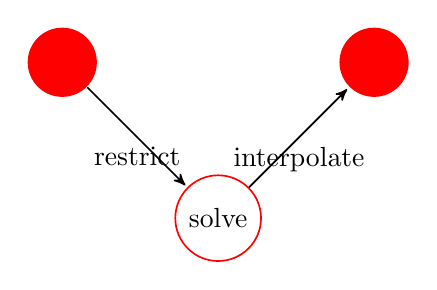
\begin{tikzpicture}[->,>=stealth',shorten >=1pt,auto,node distance=2.8cm,semithick]
                  \tikzstyle{every state}=[fill=red,draw=none,text=white]

                  \node[state]         (A)                    {};
                  \node[state,fill=none,draw=red,text=black]         (B) [below right of=A] {solve};
                  \node[state]         (C) [above right of=B] {};

                  \path (A) edge  node[below] {restrict} (B)
                        (B) edge  node[below] {interpolate} (C);
                \end{tikzpicture}
            \end{center}
        \subsubsection{3-Grid}
            MG Iteration
            \begin{itemize}
                \item Smooth $\nu_1$ times
                \item Compute $r_h$
                \begin{itemize}
                    \item restrict to $f_{2h}$
                    \item solve $L_{2h}e_{2h} = r_{2h}$
                    \item smooth $L_{2h}u_{2h} = f_{2h}$, $\nu_1$ times, initial guess $e_{2h} \approx 0$.
                    \item compute $r_{2h}$
                    \begin{itemize}
                        \item Restrict to $f_{4h}$
                        \item SOlve $L_{4h}u_{4h} = f_{4h}$
                    \end{itemize}
                    \item iterpolate and correct $u_{2h} = u_{2h} + I_{4h}^{2h}u_{4h}$
                    \item smooth $\nu_2$ times
                \end{itemize}
                \item interpolate and correct $u_h = u_h + I_{2h}^hu_{2h}$
                \item Smooth $\nu_2$ times
            \end{itemize}
            \begin{center}
                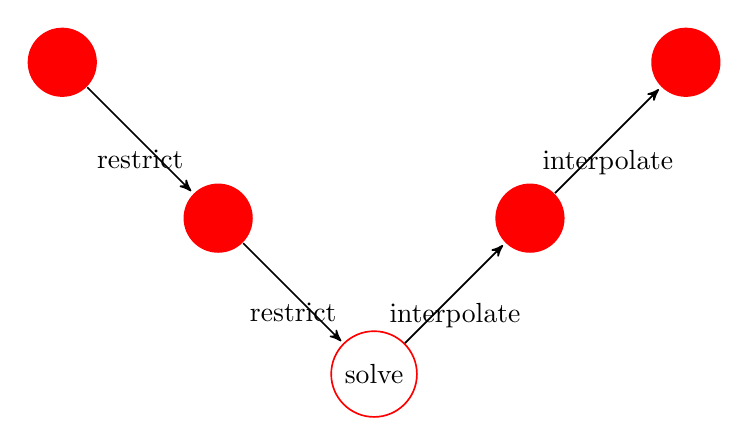
\begin{tikzpicture}[->,>=stealth',shorten >=1pt,auto,node distance=2.8cm,semithick]
                  \tikzstyle{every state}=[fill=red,draw=none,text=white]

                  \node[state]         (A)                    {};
                  \node[state]         (B) [below right of=A] {};
                  \node[state,fill=none,draw=red,text=black]         (C) [below right of=B] {solve};
                  \node[state]         (D) [above right of=C] {};
                  \node[state]         (E) [above right of=D] {};

                  \path (A) edge  node[below] {restrict} (B)
                        (B) edge  node[below] {restrict} (C)
                        (C) edge  node[below] {interpolate} (D)
                        (D) edge  node[below] {interpolate} (E);
                \end{tikzpicture}
            \end{center}
        \subsubsection{Other forms of cycles}
            Do $\gamma$ iteration before returning to fine grid. $\gamma = 1$ is called $V$-cycle, $\gamma=2$ for three grids is called $W$-cycle.  $\gamma=2$ for 3 levels looks like
            \begin{center}
                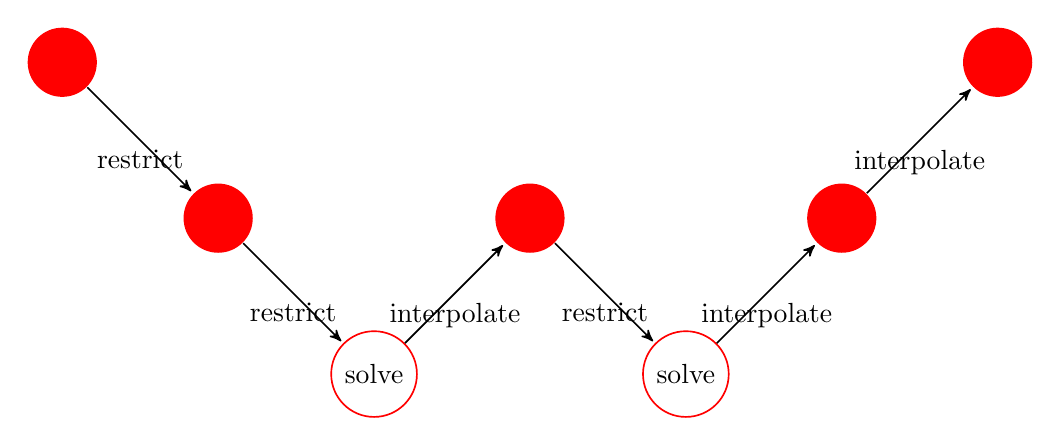
\begin{tikzpicture}[->,>=stealth',shorten >=1pt,auto,node distance=2.8cm,semithick]
                  \tikzstyle{every state}=[fill=red,draw=none,text=white]

                  \node[state]         (A)                    {};
                  \node[state]         (B) [below right of=A] {};
                  \node[state,fill=none,draw=red,text=black]         (C) [below right of=B] {solve};
                  \node[state]         (D) [above right of=C] {};
                  \node[state,fill=none,draw=red,text=black]         (E) [below right of=D] {solve};
                  \node[state]         (F) [above right of=E] {};
                  \node[state]         (G) [above right of=F] {};

                  \path (A) edge  node[below] {restrict} (B)
                        (B) edge  node[below] {restrict} (C)
                        (C) edge  node[below] {interpolate} (D)
                        (D) edge  node[below] {restrict} (E)
                        (E) edge  node[below] {interpolate} (F)
                        (F) edge  node[below] {interpolate} (G);
                \end{tikzpicture}
            \end{center}
            \FloatBarrier
            $\gamma=2$ for $4$ levels looks like a fractal.
        \subsubsection{How much work is there in a $V$-cycle?}
            On the fine mesh, smooth, $\nu$ times is $\order{N}$.  We also have to compute the residual, $r_h = \order{N}$.  We also have to restrict, $\order{N}$.  We also have to correct $\order{N}$ and interpolate $\order{N}$. \\

            In 2D, the work on a fine mesh is $CN$.  Every time we drop a level is dropping by a factor of $4$..
            \begin{align*}
                \begin{array}{||c|c||}\hline\hline
                    \text{level $\ell$} & \text{work} \\\hline\hline
                    \ell=1 & CN \\\hline
                    \ell=2 & \dfrac{CN}{4} \\\hline
                    \ell=3 & \dfrac{CN}{4^2} \\\hline
                    \vdots & \vdots \\\hline\hline
                \end{array}
            \end{align*}
            The total work in the limit of many levels is
            \begin{align*}
                \sum_{\ell=1}^L CN\qty(\frac{1}{4})^{\ell-1} \approx CN\qty(\frac{1}{1 - \frac{1}{4}}) = \frac{4}{3}CN
            \end{align*}
            So $V$-cycle work is not much different than work on the fine level.
    \subsection{GS-RB, FM, bilinear interpolation, 2D}
        For $\nu=2$, 2-grid gives $\rho\approx0.074$.  $V$-cycle gives $\rho\approx0.10$.

    \subsection{Comparisons to SOR}
        Say we have $64\times64$ mesh with tolerance of $10^{-6}$.
        \begin{align*}
            \begin{array}{||c|c|c|c||}\hline\hline
                & \text{\# iterations} & \text{work per iteration} & \text{total work} \\\hline\hline
                \text{SOR} & 144 & 1 & 144 \\\hline
                \text{MG} & 6 & \nicefrac{4}{3}\cdot\qty(2 + 4) = 8 & 48 \\\hline\hline
            \end{array}
        \end{align*}
        Say we have $265\times265$ mesh with tolerance of $10^{-7}$.
        \begin{align*}
            \begin{array}{||c|c|c|c||}\hline\hline
                & \text{\# iterations} & \text{work per iteration} & \text{total work} \\\hline\hline
                \text{SOR} & 658 & 1 & 658 \\\hline
                \text{MG} & 7 & \nicefrac{4}{3}\cdot\qty(2 + 4) = 8 & 56 \\\hline\hline
            \end{array}
        \end{align*}

\end{document}



















